
%% bare_conf.tex
%% V1.3
%% 2007/01/11
%% by Michael Shell
%% See:
%% http://www.michaelshell.org/
%% for current contact information.
%%
%% This is a skeleton file demonstrating the use of IEEEtran.cls
%% (requires IEEEtran.cls version 1.7 or later) with an IEEE conference paper.
%%
%% Support sites:
%% http://www.michaelshell.org/tex/ieeetran/
%% http://www.ctan.org/tex-archive/macros/latex/contrib/IEEEtran/
%% and
%% http://www.ieee.org/

%%*************************************************************************
%% Legal Notice:
%% This code is offered as-is without any warranty either expressed or
%% implied; without even the implied warranty of MERCHANTABILITY or
%% FITNESS FOR A PARTICULAR PURPOSE!
%% User assumes all risk.
%% In no event shall IEEE or any contributor to this code be liable for
%% any damages or losses, including, but not limited to, incidental,
%% consequential, or any other damages, resulting from the use or misuse
%% of any information contained here.
%%
%% All comments are the opinions of their respective authors and are not
%% necessarily endorsed by the IEEE.
%%
%% This work is distributed under the LaTeX Project Public License (LPPL)
%% ( http://www.latex-project.org/ ) version 1.3, and may be freely used,
%% distributed and modified. A copy of the LPPL, version 1.3, is included
%% in the base LaTeX documentation of all distributions of LaTeX released
%% 2003/12/01 or later.
%% Retain all contribution notices and credits.
%% ** Modified files should be clearly indicated as such, including  **
%% ** renaming them and changing author support contact information. **
%%
%% File list of work: IEEEtran.cls, IEEEtran_HOWTO.pdf, bare_adv.tex,
%%                    bare_conf.tex, bare_jrnl.tex, bare_jrnl_compsoc.tex
%%*************************************************************************

% *** Authors should verify (and, if needed, correct) their LaTeX system  ***
% *** with the testflow diagnostic prior to trusting their LaTeX platform ***
% *** with production work. IEEE's font choices can trigger bugs that do  ***
% *** not appear when using other class files.                            ***
% The testflow support page is at:
% http://www.michaelshell.org/tex/testflow/



% Note that the a4paper option is mainly intended so that authors in
% countries using A4 can easily print to A4 and see how their papers will
% look in print - the typesetting of the document will not typically be
% affected with changes in paper size (but the bottom and side margins will).
% Use the testflow package mentioned above to verify correct handling of
% both paper sizes by the user's LaTeX system.
%
% Also note that the "draftcls" or "draftclsnofoot", not "draft", option
% should be used if it is desired that the figures are to be displayed in
% draft mode.
%
\documentclass[conference]{IEEEtran}
\usepackage{blindtext, graphicx}
\usepackage[utf8]{inputenc}
\usepackage[english, slovenian]{babel}
%\usepackage[active,displaymath,tightpage]{preview}
%\setlength\PreviewBorder{1em}
% Add the compsoc option for Computer Society conferences.
%
% If IEEEtran.cls has not been installed into the LaTeX system files,
% manually specify the path to it like:
% \documentclass[conference]{../sty/IEEEtran}


\usepackage{caption}
\captionsetup[table]{skip=10pt}


\usepackage{graphicx}
\usepackage{subcaption}
\usepackage{float}

% Some very useful LaTeX packages include:
% (uncomment the ones you want to load)


% *** MISC UTILITY PACKAGES ***
%
%\usepackage{ifpdf}
% Heiko Oberdiek's ifpdf.sty is very useful if you need conditional
% compilation based on whether the output is pdf or dvi.
% usage:
% \ifpdf
%   % pdf code
% \else
%   % dvi code
% \fi
% The latest version of ifpdf.sty can be obtained from:
% http://www.ctan.org/tex-archive/macros/latex/contrib/oberdiek/
% Also, note that IEEEtran.cls V1.7 and later provides a builtin
% \ifCLASSINFOpdf conditional that works the same way.
% When switching from latex to pdflatex and vice-versa, the compiler may
% have to be run twice to clear warning/error messages.






% *** CITATION PACKAGES ***
%
%\usepackage{cite}
% cite.sty was written by Donald Arseneau
% V1.6 and later of IEEEtran pre-defines the format of the cite.sty package
% \cite{} output to follow that of IEEE. Loading the cite package will
% result in citation numbers being automatically sorted and properly
% "compressed/ranged". e.g., [1], [9], [2], [7], [5], [6] without using
% cite.sty will become [1], [2], [5]--[7], [9] using cite.sty. cite.sty's
% \cite will automatically add leading space, if needed. Use cite.sty's
% noadjust option (cite.sty V3.8 and later) if you want to turn this off.
% cite.sty is already installed on most LaTeX systems. Be sure and use
% version 4.0 (2003-05-27) and later if using hyperref.sty. cite.sty does
% not currently provide for hyperlinked citations.
% The latest version can be obtained at:
% http://www.ctan.org/tex-archive/macros/latex/contrib/cite/
% The documentation is contained in the cite.sty file itself.






% *** GRAPHICS RELATED PACKAGES ***
%
\ifCLASSINFOpdf
  % \usepackage[pdftex]{graphicx}
  % declare the path(s) where your graphic files are
  % \graphicspath{{../pdf/}{../jpeg/}}
  % and their extensions so you won't have to specify these with
  % every instance of \includegraphics
  % \DeclareGraphicsExtensions{.pdf,.jpeg,.png}
\else
  % or other class option (dvipsone, dvipdf, if not using dvips). graphicx
  % will default to the driver specified in the system graphics.cfg if no
  % driver is specified.
  % \usepackage[dvips]{graphicx}
  % declare the path(s) where your graphic files are
  % \graphicspath{{../eps/}}
  % and their extensions so you won't have to specify these with
  % every instance of \includegraphics
  % \DeclareGraphicsExtensions{.eps}
\fi
% graphicx was written by David Carlisle and Sebastian Rahtz. It is
% required if you want graphics, photos, etc. graphicx.sty is already
% installed on most LaTeX systems. The latest version and documentation can
% be obtained at:
% http://www.ctan.org/tex-archive/macros/latex/required/graphics/
% Another good source of documentation is "Using Imported Graphics in
% LaTeX2e" by Keith Reckdahl which can be found as epslatex.ps or
% epslatex.pdf at: http://www.ctan.org/tex-archive/info/
%
% latex, and pdflatex in dvi mode, support graphics in encapsulated
% postscript (.eps) format. pdflatex in pdf mode supports graphics
% in .pdf, .jpeg, .png and .mps (metapost) formats. Users should ensure
% that all non-photo figures use a vector format (.eps, .pdf, .mps) and
% not a bitmapped formats (.jpeg, .png). IEEE frowns on bitmapped formats
% which can result in "jaggedy"/blurry rendering of lines and letters as
% well as large increases in file sizes.
%
% You can find documentation about the pdfTeX application at:
% http://www.tug.org/applications/pdftex





% *** MATH PACKAGES ***
%
%\usepackage[cmex10]{amsmath}
% A popular package from the American Mathematical Society that provides
% many useful and powerful commands for dealing with mathematics. If using
% it, be sure to load this package with the cmex10 option to ensure that
% only type 1 fonts will utilized at all point sizes. Without this option,
% it is possible that some math symbols, particularly those within
% footnotes, will be rendered in bitmap form which will result in a
% document that can not be IEEE Xplore compliant!
%
% Also, note that the amsmath package sets \interdisplaylinepenalty to 10000
% thus preventing page breaks from occurring within multiline equations. Use:
%\interdisplaylinepenalty=2500
% after loading amsmath to restore such page breaks as IEEEtran.cls normally
% does. amsmath.sty is already installed on most LaTeX systems. The latest
% version and documentation can be obtained at:
% http://www.ctan.org/tex-archive/macros/latex/required/amslatex/math/





% *** SPECIALIZED LIST PACKAGES ***
%
%\usepackage{algorithmic}
% algorithmic.sty was written by Peter Williams and Rogerio Brito.
% This package provides an algorithmic environment fo describing algorithms.
% You can use the algorithmic environment in-text or within a figure
% environment to provide for a floating algorithm. Do NOT use the algorithm
% floating environment provided by algorithm.sty (by the same authors) or
% algorithm2e.sty (by Christophe Fiorio) as IEEE does not use dedicated
% algorithm float types and packages that provide these will not provide
% correct IEEE style captions. The latest version and documentation of
% algorithmic.sty can be obtained at:
% http://www.ctan.org/tex-archive/macros/latex/contrib/algorithms/
% There is also a support site at:
% http://algorithms.berlios.de/index.html
% Also of interest may be the (relatively newer and more customizable)
% algorithmicx.sty package by Szasz Janos:
% http://www.ctan.org/tex-archive/macros/latex/contrib/algorithmicx/




% *** ALIGNMENT PACKAGES ***
%
%\usepackage{array}
% Frank Mittelbach's and David Carlisle's array.sty patches and improves
% the standard LaTeX2e array and tabular environments to provide better
% appearance and additional user controls. As the default LaTeX2e table
% generation code is lacking to the point of almost being broken with
% respect to the quality of the end results, all users are strongly
% advised to use an enhanced (at the very least that provided by array.sty)
% set of table tools. array.sty is already installed on most systems. The
% latest version and documentation can be obtained at:
% http://www.ctan.org/tex-archive/macros/latex/required/tools/


%\usepackage{mdwmath}
%\usepackage{mdwtab}
% Also highly recommended is Mark Wooding's extremely powerful MDW tools,
% especially mdwmath.sty and mdwtab.sty which are used to format equations
% and tables, respectively. The MDWtools set is already installed on most
% LaTeX systems. The lastest version and documentation is available at:
% http://www.ctan.org/tex-archive/macros/latex/contrib/mdwtools/


% IEEEtran contains the IEEEeqnarray family of commands that can be used to
% generate multiline equations as well as matrices, tables, etc., of high
% quality.


%\usepackage{eqparbox}
% Also of notable interest is Scott Pakin's eqparbox package for creating
% (automatically sized) equal width boxes - aka "natural width parboxes".
% Available at:
% http://www.ctan.org/tex-archive/macros/latex/contrib/eqparbox/





% *** SUBFIGURE PACKAGES ***
%\usepackage[tight,footnotesize]{subfigure}
% subfigure.sty was written by Steven Douglas Cochran. This package makes it
% easy to put subfigures in your figures. e.g., "Figure 1a and 1b". For IEEE
% work, it is a good idea to load it with the tight package option to reduce
% the amount of white space around the subfigures. subfigure.sty is already
% installed on most LaTeX systems. The latest version and documentation can
% be obtained at:
% http://www.ctan.org/tex-archive/obsolete/macros/latex/contrib/subfigure/
% subfigure.sty has been superceeded by subfig.sty.



%\usepackage[caption=false]{caption}
%\usepackage[font=footnotesize]{subfig}
% subfig.sty, also written by Steven Douglas Cochran, is the modern
% replacement for subfigure.sty. However, subfig.sty requires and
% automatically loads Axel Sommerfeldt's caption.sty which will override
% IEEEtran.cls handling of captions and this will result in nonIEEE style
% figure/table captions. To prevent this problem, be sure and preload
% caption.sty with its "caption=false" package option. This is will preserve
% IEEEtran.cls handing of captions. Version 1.3 (2005/06/28) and later
% (recommended due to many improvements over 1.2) of subfig.sty supports
% the caption=false option directly:
%\usepackage[caption=false,font=footnotesize]{subfig}
%
% The latest version and documentation can be obtained at:
% http://www.ctan.org/tex-archive/macros/latex/contrib/subfig/
% The latest version and documentation of caption.sty can be obtained at:
% http://www.ctan.org/tex-archive/macros/latex/contrib/caption/




% *** FLOAT PACKAGES ***
%
%\usepackage{fixltx2e}
% fixltx2e, the successor to the earlier fix2col.sty, was written by
% Frank Mittelbach and David Carlisle. This package corrects a few problems
% in the LaTeX2e kernel, the most notable of which is that in current
% LaTeX2e releases, the ordering of single and double column floats is not
% guaranteed to be preserved. Thus, an unpatched LaTeX2e can allow a
% single column figure to be placed prior to an earlier double column
% figure. The latest version and documentation can be found at:
% http://www.ctan.org/tex-archive/macros/latex/base/



%\usepackage{stfloats}
% stfloats.sty was written by Sigitas Tolusis. This package gives LaTeX2e
% the ability to do double column floats at the bottom of the page as well
% as the top. (e.g., "\begin{figure*}[!b]" is not normally possible in
% LaTeX2e). It also provides a command:
%\fnbelowfloat
% to enable the placement of footnotes below bottom floats (the standard
% LaTeX2e kernel puts them above bottom floats). This is an invasive package
% which rewrites many portions of the LaTeX2e float routines. It may not work
% with other packages that modify the LaTeX2e float routines. The latest
% version and documentation can be obtained at:
% http://www.ctan.org/tex-archive/macros/latex/contrib/sttools/
% Documentation is contained in the stfloats.sty comments as well as in the
% presfull.pdf file. Do not use the stfloats baselinefloat ability as IEEE
% does not allow \baselineskip to stretch. Authors submitting work to the
% IEEE should note that IEEE rarely uses double column equations and
% that authors should try to avoid such use. Do not be tempted to use the
% cuted.sty or midfloat.sty packages (also by Sigitas Tolusis) as IEEE does
% not format its papers in such ways.





% *** PDF, URL AND HYPERLINK PACKAGES ***
%
%\usepackage{url}
% url.sty was written by Donald Arseneau. It provides better support for
% handling and breaking URLs. url.sty is already installed on most LaTeX
% systems. The latest version can be obtained at:
% http://www.ctan.org/tex-archive/macros/latex/contrib/misc/
% Read the url.sty source comments for usage information. Basically,
% \url{my_url_here}.





% *** Do not adjust lengths that control margins, column widths, etc. ***
% *** Do not use packages that alter fonts (such as pslatex).         ***
% There should be no need to do such things with IEEEtran.cls V1.6 and later.
% (Unless specifically asked to do so by the journal or conference you plan
% to submit to, of course. )


% correct bad hyphenation here
\hyphenation{op-tical net-works semi-conduc-tor}


\begin{document}
%
% paper title
% can use linebreaks \\ within to get better formatting as desired
\title{Data clustering using stochastic block models}


% author names and affiliations
% use a multiple column layout for up to three different
% affiliations
\author{\IEEEauthorblockN{Nina Mrzelj}
\IEEEauthorblockA{University of Ljubljana, \\
Faculty of Mathematics and Physics\\
Email: nina.mrzelj@gmail.com}
\and

\IEEEauthorblockN{Pavlin Gregor Poličar}
\IEEEauthorblockA{ University of Ljubljana,\\
Faculty of Computer and Information Science\\
Email: pavlin.g.p@gmail.com}}

% conference papers do not typically use \thanks and this command
% is locked out in conference mode. If really needed, such as for
% the acknowledgment of grants, issue a \IEEEoverridecommandlockouts
% after \documentclass

% for over three affiliations, or if they all won't fit within the width
% of the page, use this alternative format:
%
%\author{\IEEEauthorblockN{Michael Shell\IEEEauthorrefmark{1},
%Homer Simpson\IEEEauthorrefmark{2},
%James Kirk\IEEEauthorrefmark{3},
%Montgomery Scott\IEEEauthorrefmark{3} and
%Eldon Tyrell\IEEEauthorrefmark{4}}
%\IEEEauthorblockA{\IEEEauthorrefmark{1}School of Electrical and Computer Engineering\\
%Georgia Institute of Technology,
%Atlanta, Georgia 30332--0250\\ Email: see http://www.michaelshell.org/contact.html}
%\IEEEauthorblockA{\IEEEauthorrefmark{2}Twentieth Century Fox, Springfield, USA\\
%Email: homer@thesimpsons.com}
%\IEEEauthorblockA{\IEEEauthorrefmark{3}Starfleet Academy, San Francisco, California 96678-2391\\
%Telephone: (800) 555--1212, Fax: (888) 555--1212}
%\IEEEauthorblockA{\IEEEauthorrefmark{4}Tyrell Inc., 123 Replicant Street, Los Angeles, California 90210--4321}}




% use for special paper notices
%\IEEEspecialpapernotice{(Invited Paper)}




% make the title area
\maketitle


\begin{abstract}
%\boldmath
It has been shown that community detection algorithms work better for clustering tasks than other, more popular methods, such as k-means. In fact, network analysis based methods often outperform more widely used methods and do not suffer from some of the drawbacks we notice elsewhere e.g. the number of clusters $k$ usually has to be known in advance. However, stochastic block models which are known to perform well for community detection, have not yet been tested for this task. We discuss why these models cannot be directly applied to this problem and test the performance of a generalization of stochastic block models which work on weighted graphs and compare them to other clustering techniques.
\end{abstract}
% IEEEtran.cls defaults to using nonbold math in the Abstract.
% This preserves the distinction between vectors and scalars. However,
% if the journal you are submitting to favors bold math in the abstract,
% then you can use LaTeX's standard command \boldmath at the very start
% of the abstract to achieve this. Many IEEE journals frown on math
% in the abstract anyway.

% Note that keywords are not normally used for peerreview papers.
% \begin{IEEEkeywords}
% Clustering, stochastic block models,
% \end{IEEEkeywords}






% For peer review papers, you can put extra information on the cover
% page as needed:
% \ifCLASSOPTIONpeerreview
% \begin{center} \bfseries EDICS Category: 3-BBND \end{center}
% \fi
%
% For peerreview papers, this IEEEtran command inserts a page break and
% creates the second title. It will be ignored for other modes.
\IEEEpeerreviewmaketitle

\section{Introduction}
Clustering methods are one of the fundamental topics in machine learning since they can be used to detect structure in unlabelled data. As this is such a broadly applicable task, many solutions have been proposed~\cite{theodoridis2003pattern}, the most popular of which is k-means~\cite{macqueen1967some}, due to its simplicity, fast execution time and good performance. However, k-means and other traditional machine learning approaches to clustering suffer from certain drawbacks. In many cases, the number of clusters $k$ must be predefined i.e. we must know in advance how many clusters appear in the data. Furthermore, most of these techniques produce clusters of circular geometric shapes (this is especially true for k-means). These are both undesirable properties, since we can rarely know the correct number of clusters in advance, or that clusters appear in a particular shape.

The idea to use community detection algorithms for the clustering task was first proposed in 2008~\cite{de2008data}. The suggested approach was robust in finding clusters of different shapes, but the number of clusters still had to be provided. However, the authors considered only a single community detection algorithm with a single metric.
% TODO Describe what rodrigues did in his work: Please briefly describe what the authors did, and also what are community detection methods and why one has to decide for a certain metric. This might not be immediately clear to a reader that is not familiar with the topic.

In the work of Rodrigues et al.~\cite{rodrigues2011complex}, other community detection algorithms were considered with a variety of metrics. It was shown that certain community detection algorithms almost always outperform more traditional methods and that some of these approaches do not suffer from the aforementioned drawbacks of other methods. In particular, they showed that using Manhattan or Chebyshev dissimilarity is most suitable for complex network approaches for clustering. The smallest misclassification rates were achieved with a community detection method based on greedy modularity optimization.

We extend the research done by Rodrigues et al. with stochastic block models \cite{holland1983stochastic}, which are also known to work well for community detection tasks in the scope of network analysis~\cite{fortunato2010community}. We discuss the difficulties that arise when trying to apply these models to such data and provide a solution. We also solve the clustering task using a generalization of stochastic block models that support weighted graphs~\cite{aicher2013adapting}. We evaluate the performance of these models with a series of classification tasks, both on synthetic and real-world datasets and compare them to other complex network based methods, as well as more traditional clustering techniques.

\section{Concepts and methods}

Stochastic block models are known to work well for community detection and can reveal many forms of network structure, so naturally, we expect it to also work well for data clustering. However, they cannot be directly applied to clustering problems, since they cannot account for edge weights, which are the central element of clustering using a complex networks approach.

\subsection{Stochastic block models}

The stochastic block model (SBM)~\cite{holland1983stochastic} is a generative model for learning community structure in unweighted networks. The model assigns each node $i$ to one of $K$ blocks denoted by $z_i$, and each each edge $A_{ij}$ exists with a probability $\theta_{z_i z_j}$ where $\theta$ is a $K \times K$ matrix which values are the probabilities of links appearing between blocks $i$ and $j$. The optimal block assignment is selected using a probabilistic maximum likelihood approach.

The stochastic block model can generate a wide variety of patterns that appear in network analysis including assortative, disassortative and core-periphery structures. However, this probabilistic model assumes an unweighted network. To remedy this, weighted networks are most often simplified into unweighted networks by applying a single global threshold.

This is problematic, since Aicher et al.~\cite{aicher2013adapting} showed that there are cases where this approach will never yield the correct block structure for any thershold value. Applying a single global threshold completely discards any local information that may be encoded within the edge weights. They propose a generalization of the stochastic block model, the weighted stochastic block model (WSBM) which removes the need for thresholding altogether. The model assumes that the weights are exponentially distributed and accepts a parameter $\alpha$ which balances the information gained from a missing edge and an edge with zero weight.

\subsection{Representing tabular data as a network}

The first step of any clustering using complex networks approaches requires the tabular data to be represented as a graph. A full graph is induced from the data. Each vertex represents a data point and their distances to other nodes are represented as the weights on the corresponding edges. Since the space of possible metrics is vast, we limit ourselves to the following metrics:

% TODO These formulae seem super excessive... Perhaps we could just point out that they are just Minkwoski distances with different values of p
\begin{enumerate}
    \item Exponential of Chebyshev distance
    $$ S_C(x,y) = {\textnormal{exp}( - max_{i = 1}^n \left | x_i - y_i \right | )} $$

    \item Exponential of Manhattan distance
    $$ S_M(x,y) = \textnormal{exp} \Big ( -\sum_{i=1}^{n} \left | x_i - y_i \right | \Big)$$

    \item Exponential of Euclidean distance
    $$ S_E(x,y) = \textnormal{exp} \Big ( - \big ( \sum_{i=1}^{n} \left ( x_i - y_i \right ) ^2 \big ) ^{\frac{1}{2}} \Big) $$

\end{enumerate}

In the formulae above, $x, y \in {\rm I\!R}^n$ denote data points with $n$ features. Metrics 1 and 2 are chosen because were shown to produce small error rates in work of Rodrigues et al.~\cite{rodrigues2011complex}. In networks, where these two measures work poorly, we also consider the exponential of Euclidean distance.

We only consider exponential distances since they have the desirable property of being limited to the interval $\left [ 0, 1 \right ]$. Moreover, a larger exponential distance indicates greater similarity, whereas the opposite is true for their non-exponential versions. This is conceptually more sound, since we would intuitively assign larger values to data points which are more similar.

Using only the exponential variants of the distance metrics, we also satisfy the requirement imposed by the WSBM: that the edge weights in a network must be exponentially distributed.

We can now directly use the induced graphs with algorithms that can take edge weights into account, such as the WSBM. However, the classic SBM cannot do this, therefore a preprocessing step is required to remove a number of edges, so that the model may find any meaningful structure within the data. Were we to ignore this step, the model would find a single block containing all the nodes. The simplest solution is to apply a single global threshold to all the edges, and to apply the model to the pruned graph. We describe this approach in the following section.

\subsection{Determine the optimal cutoff threshold}

Before we can apply the classic SBM~\cite{karrer2011stochastic} on the graph, we must first find an appropriate threshold, so that the model may find any meaningful structure. However, finding such a threshold so that optimal clustering is achieved is not trivial. Figure~\ref{fig:iris_graph} shows the induced graph on the well-known Iris dataset for three different threshold values. We expect that the SBM may be able to detect the correct block structure for all three values of the cutoff rate.

\begin{figure}[H]
    \centering
    \begin{subfigure}[c]{\columnwidth}
        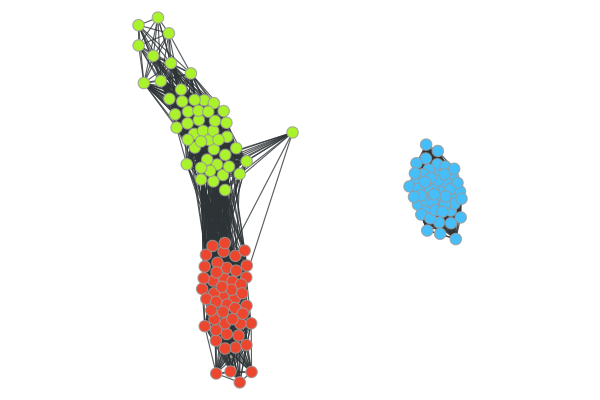
\includegraphics[width=\columnwidth]{images/iris_threshold_01.png}
        \caption{Threshold of 0.1}
        \label{fig:iris_graph1}
    \end{subfigure}
    ~
    \begin{subfigure}[c]{\columnwidth}
        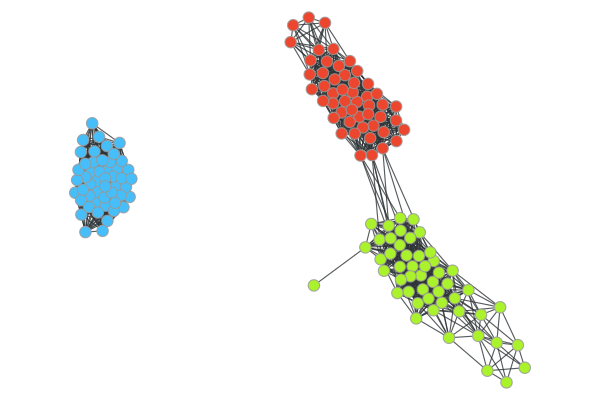
\includegraphics[width=\columnwidth]{images/iris_threshold_02.png}
        \caption{Threshold of 0.2}
        \label{fig:iris_graph2}
    \end{subfigure}
    ~
    \begin{subfigure}[c]{\columnwidth}
        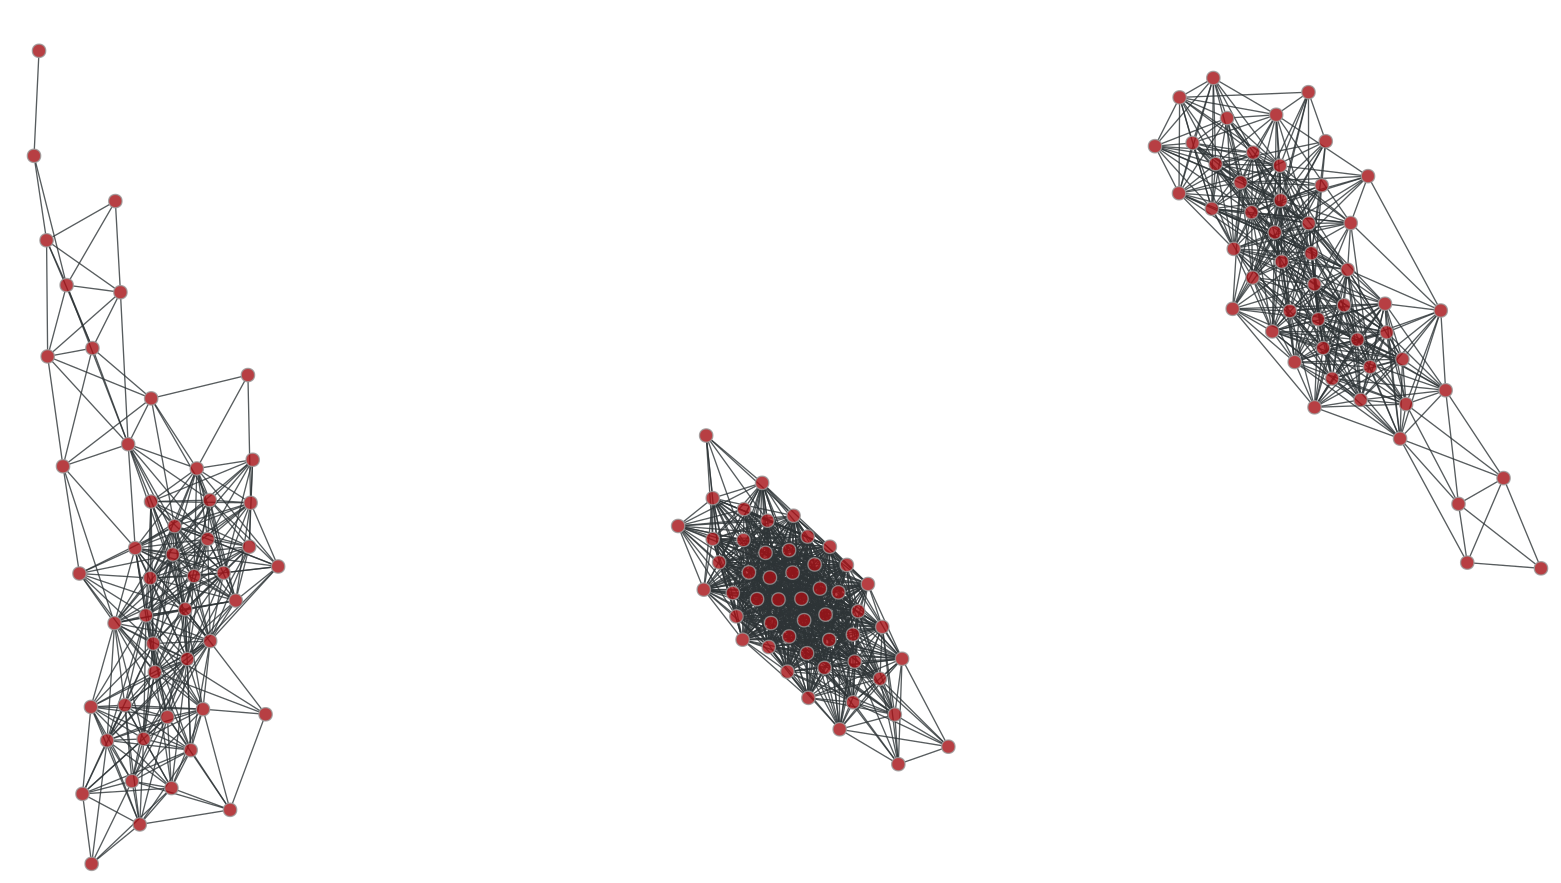
\includegraphics[width=\columnwidth]{images/iris_threshold_03.png}
        \caption{Threshold of 0.3}
        \label{fig:iris_graph3}
    \end{subfigure}
    \caption{The induced graph of the Iris dataset with a three different global thresholds. The dataset contains three distinct classes, which are clearly separated in the above images.}\label{fig:iris_graph}
\end{figure}

This can be translated into the classical problem that other traditional clustering methods face, when the optimal number of clusters cannot be inferred automatically by the algorithm or is not known. We evaluate cluster labelling for different thresholds using the silhouette score (see Equation~\ref{eq:silhouette}) - a popular evaluation metric for evaluating clustering quality.

\begin{equation}\label{eq:silhouette}
s(i) = \frac{{b(i) - a(i)}}{\max\{a(i),b(i)\}}
\end{equation}

The silhouette score is calculated with $a(i)$, which denotes the mean intra-cluster distance from point $i$ to all other points within that same cluster, and $b(i)$, which denotes the mean distance from point $i$ to all points within the nearest cluster to point $i$.

However, when the true cluster labels are known, we can use the more informative mutual information score or NMI (see Equation~\ref{eq:nmi}).

\begin{equation}\label{eq:nmi}
\textnormal{NMI}(T, C) = \frac{2 \, I(T, C)}{H(T) + H(C)}
\end{equation}

The NMI considers the mutual information $I$ of two clusterings: the true labels $T$ and our computed labels $C$. This is then normalized by the sum of their entropies $H$.  This score is a better indicator of the actual success rate of the method, since it also takes into account the true labels of the data.

%% TODO Ali je ta sestavek sploh smiselen, glede na to da se silhoueta uporabla povsod drugot
By comparing the NMI and silhouette scores on the same datasets, we verify that indeed, the silhouette score is a good indicator of clustering quality (see Figure~\ref{fig:threshold_sbm_iris_nmi_slh}). They do not overlap, which is to be expected, as the scores have different bounds. However, it is clear that the optimal value is achieved at the same threshold value, therefore we can conclude that the silhouette score is a reliable indicator of cluster quality (this test was run on several datasets, but we include only one for illustrative purposes).

\begin{figure}[ht]
    \centering
    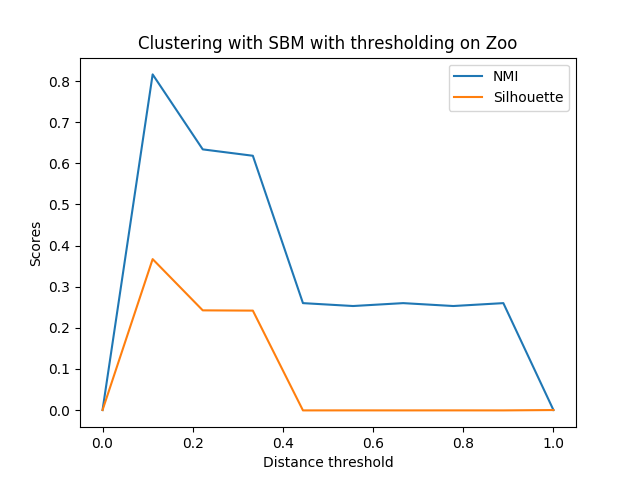
\includegraphics[width=0.9\columnwidth]{results/threshold_clustering_zoo.png}
    \caption{A comparison of silhouette scores and NMI scores on the Zoo dataset~\cite{Lichman:2013}.}
    \label{fig:threshold_sbm_iris_nmi_slh}
\end{figure}


%% TODO This has to go in its own section, since the work done above all includes sbm with different thresholds
%With different values for the threshold, we can force the network to degrade into $k$ connected components. We can now use these connected components as labels for the different clusters. This is similar to single linkage hierarchical clustering, but using a top-down approach. Of course, we must still determine the optimal value for $k$, which we select based on the silhouette score (see Equation \ref{eq:silhouette}) for different threshold values.


\section{Results and discussion}

We evaluate the proposed clustering techniques on five real-world datasets from the UCI Machine Learning Repository~\cite{Lichman:2013}: Iris, Ecoli, Glass, Zoo and Movements. We also test the methods on three synthetic datasets: two moons, circles and the INA dataset (shown in Figure~\ref{fig:synthetic_datasets}).

\begin{figure}[H]
    \centering
    \begin{subfigure}[c]{0.3\columnwidth}
        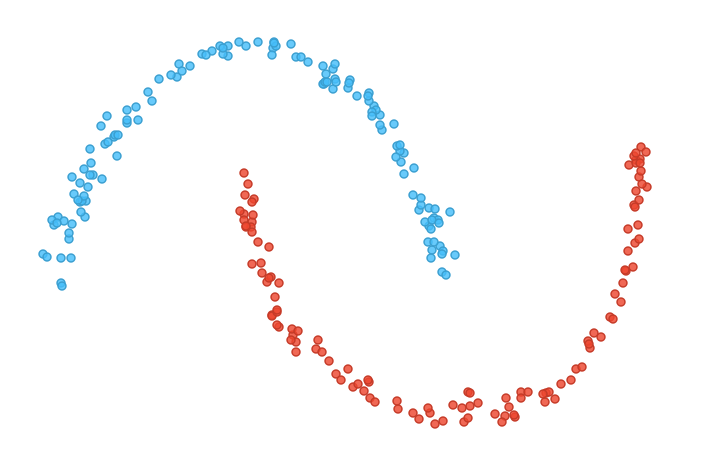
\includegraphics[width=\columnwidth]{images/moons.png}
        \caption{Two moons}
        \label{fig:synthetic_two_moons}
    \end{subfigure}
    ~
    \begin{subfigure}[c]{0.3\columnwidth}
        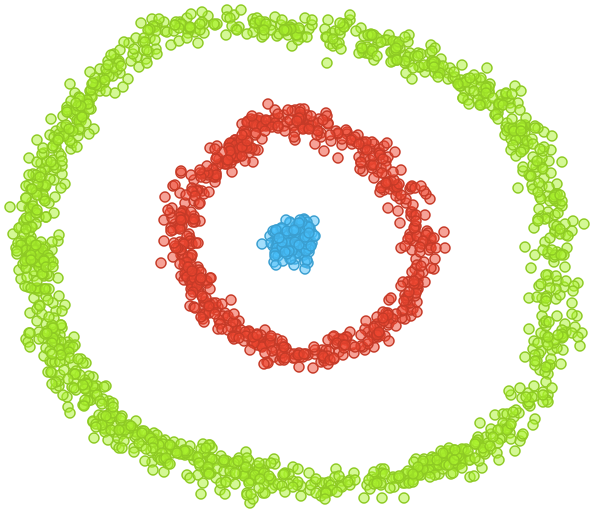
\includegraphics[width=\columnwidth]{images/circles.png}
        \caption{Circles}
        \label{fig:synthetic_circles}
    \end{subfigure}
    ~
    \begin{subfigure}[c]{0.3\columnwidth}
        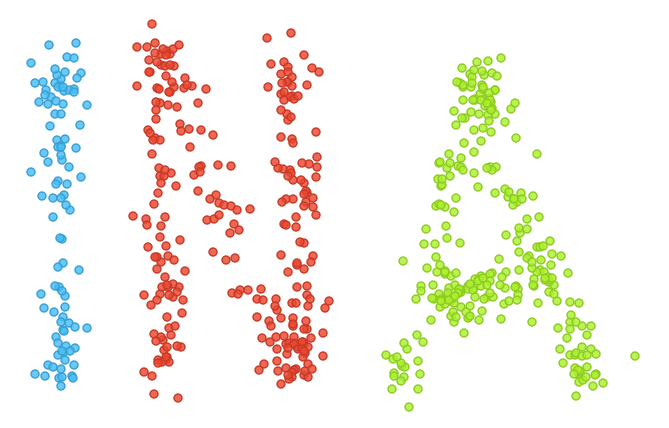
\includegraphics[width=\columnwidth]{images/ina.png}
        \caption{INA}
        \label{fig:synthetic_ina}
    \end{subfigure}
    \caption{Synthetic datasets}\label{fig:synthetic_datasets}
\end{figure}

The dataset characteristics are summarized in Table~\ref{tab:datasets}.

\begin{table}[ht]
    \centering
    \begin{tabular}{c c c c}
        Name & Instances & Features & Clusters\\ \hline
        iris & 150 & 4 & 3 \\
        ecoli & 336 & 7 & 8 \\
        glass & 214 & 9 & 6 \\
        zoo & 101 & 16 & 7 \\
        % vehicle & 846 & 18 & 4 \\
        % voting & 435 & 16 & 2 \\
        movements & 360 & 90 & 15 \\ \hline
        two moons & 250 & 2 & 2 \\
        circles & 336 & 2 & 3 \\
        ina & 660 & 2 & 3 \\
    \end{tabular}
    \caption{Description of datasets}
    \label{tab:datasets}
\end{table}


\subsection{Results}

We compare the SBM with thresholding and the WSBM with two popular clustering approaches: k-means and hierarchical clustering with Ward linkage. Since none of these methods can infer the optimal number of clusters automatically, we select the best clusterings with regard to the silhouette score.

To evaluate different clustering methods, we use three popular metrics: the adjusted Rand index or ARI~\cite{hubert1985comparing} (see Equation ~\ref{eq:ari}), normalized mutual information score (see Equation~\ref{eq:nmi}) and the silhouette score (see Equation~\ref{eq:silhouette}). The ARI is a variant of the Rand index that is corrected for chance and is used to measure the similarity between two clusterings.

\begin{equation}\label{eq:ari}
\textnormal{ARI} = \frac{RI - ExpectedRI}{max(RI) - ExpectedRI}
\end{equation}

We present the most interesting results obtained in Table~\ref{tab:results} (the full results are not included here for the sake of brevity, but the interested reader can find them in Table~\ref{tab:results_full}). We include only the variants using the Manhattan distance metric, as it gave us the best results on average. We also include the results of the WSBM where the optimal number of clusters in known in advance, again using only the Manhattan distance metric as a measure of similarity.

\begin{table}[ht]
  \centering
  \begin{tabular}{c | c | c c c | c}
    Dataset & Method & Silhouette & NMI & ARI & Clusters \\ \hline
    Iris & k-means & \textbf{0.6808} & 0.6793 & 0.5399 & 2 \\
    Iris & Hierarchical clustering & \textbf{0.6864} & \textbf{0.7612} & \textbf{0.5681} & 2 \\
    Iris & SBM & 0.3916 & 0.6752 & \textbf{0.5703} & 7 \\
    Iris & WSBM & \textbf{0.6864} & \textbf{0.7612} & \textbf{0.5681} & 2 \\
    \textit{Iris} & \textit{WSBM (known)} & \textit{0.5171} & \textit{0.7206} & \textit{0.6906} & \textit{3} \\
    \hline
    Ecoli & k-means & \textbf{0.4303} & 0.6548 & 0.6860 & 4 \\
    Ecoli & Hierarchical clustering & 0.4166 & 0.6537 & 0.6575 & 4 \\
    Ecoli & SBM & 0.0694 & 0.4821 & 0.1801 & 20 \\
    Ecoli & WSBM & 0.4263 & \textbf{0.6827} & \textbf{0.7261} & 4 \\
    \textit{Ecoli} & \textit{WSBM (known)} & \textit{0.2022} & \textit{0.5724} & \textit{0.4363} & \textit{8} \\
    \hline
    Zoo & k-means & 0.4177 & 0.8172 & \textbf{0.8418} & 6 \\
    Zoo & Hierarchical clustering & \textbf{0.4288} & \textbf{0.8485} & \textbf{0.8483} & 7 \\
    Zoo & SBM & 0.3811 & \textbf{0.8503} & 0.8137 & 5 \\
    Zoo & WSBM & 0.3191 & 0.7939 & 0.5243 & 11 \\
    \textit{Zoo} & \textit{WSBM (known)} & \textit{0.1258} & \textit{0.6229} & \textit{0.3602} & \textit{7} \\
    \hline
    % Glass & k-means & 0.5891 & 0.4409 & 0.2549 & 4 \\
    % Glass & Hierarchical clustering & 0.5888 & 0.3953 & 0.2311 & 4 \\
    % Glass & SBM & 0.1187 & 0.3546 & 0.1308 & 9 \\
    % Glass & WSBM & 0.3864 & 0.2303 & 0.1368 & 2 \\
    % % TODO Calculate this, or not, since the results are quite bad :)
    % \textit{Glass} & \textit{WSBM (known)} & \textit{?} & \textit{?} & \textit{?} & \textit{?} \\
    % \hline
    Two Moons & k-means & \textbf{0.5753} & \textbf{0.5795} & \textbf{0.2533} & 8 \\
    Two Moons & Hierarchical clustering & \textbf{0.5717} & \textbf{0.5807} & \textbf{0.2581} & 8 \\
    Two Moons & SBM & 0.5293 & 0.4944 & 0.1180 & 18 \\
    Two Moons & WSBM & \textbf{0.5692} & \textbf{0.5800} & \textbf{0.2550} & 8 \\
    \textit{Two Moons} & \textit{WSBM (known)} & \textit{0.4686} & \textit{0.2063} & \textit{0.2675} & \textit{2} \\
    \hline
    INA & k-means & \textbf{0.5466} & \textbf{0.8238} & \textbf{0.7538} & 2 \\
    INA & Hierarchical clustering  & \textbf{0.5466} & \textbf{0.8238} & \textbf{0.7538} & 2 \\
    INA & SBM & 0.4015 & 0.5468 & 0.1140 & 32 \\
    INA & WSBM & \textbf{0.5466} & \textbf{0.8238} & \textbf{0.7538} & 2 \\
    \textit{INA} & \textit{WSBM (known)} & \textit{0.4463} & \textit{0.7529} & \textit{0.6966} & \textit{3} \\
    \hline
    Circular & k-means & 0.4279 & 0.2706 & 0.0747 & 7 \\
    Circular & Hierarchical clustering & 0.4045 & 0.3324 & \textbf{0.0813} & 9 \\
    Circular & SBM & \textbf{0.5485} & \textbf{0.4901} & 0.0666 & 28 \\
    Circular & WSBM & 0.4178 & 0.3335 & \textbf{0.0894} & 8 \\
    \textit{Circular} & \textit{WSBM (known)} & \textit{0.2619} & \textit{0.2367} & \textit{0.1167} & \textit{3} \\
  \end{tabular}
  \caption{Results}
  \label{tab:results}
\end{table}

The results clearly indicate that our naive approach of applying the SBM with a simple thresholding scheme does not perform consistently. Sometimes, it outperforms the other methods by a large margin and other times, it does significantly worse. We also notice that this method most often produces a very large number of clusters.

On the other hand, the WSBM does reasonably well on most datasets, either achieving similar results to other state-of-the-art methods, while in other cases outperforming them. However, it does not show the promise of the large improvements in accuracy as presented by Rodrigues et al. The WSBM cannot fully detect the correct clusters even when the correct number of clusters is provided in advance, similarly to other techniques.

\begin{figure}[H]
    \centering
    \begin{subfigure}[c]{0.48\columnwidth}
        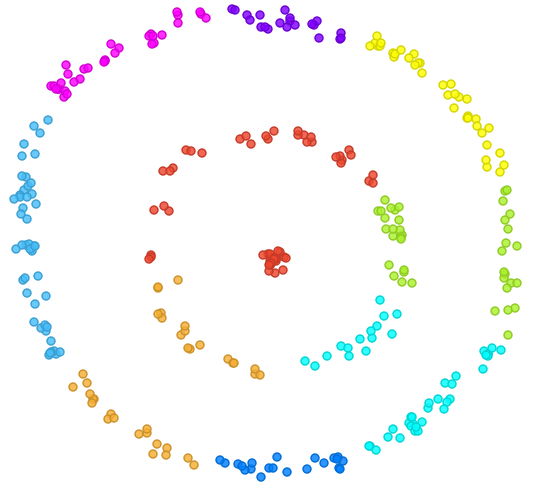
\includegraphics[width=\columnwidth]{results/circular_hc.png}
        \caption{k-means}
        \label{fig:synthetic_two_moons}
    \end{subfigure}
    ~
    \begin{subfigure}[c]{0.48\columnwidth}
        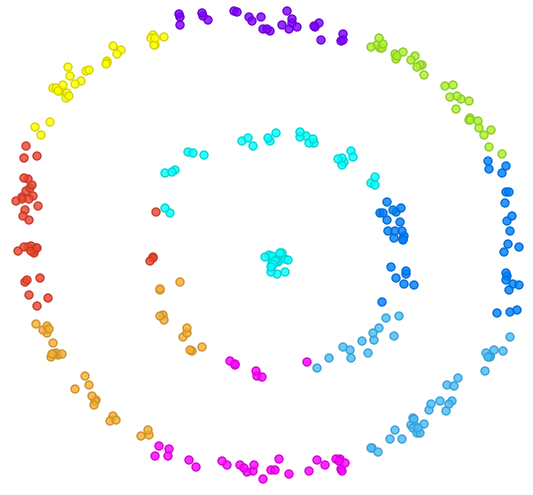
\includegraphics[width=\columnwidth]{results/circular_kmeans.png}
        \caption{Hierarchical clustering}
        \label{fig:synthetic_circles}
    \end{subfigure}
    ~
    \begin{subfigure}[c]{0.48\columnwidth}
        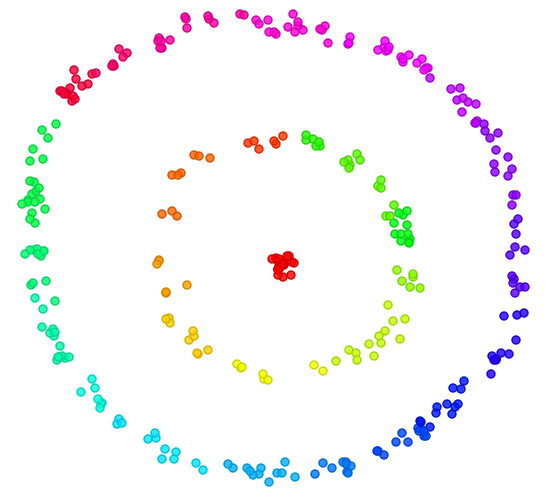
\includegraphics[width=\columnwidth]{results/circular_sbm.png}
        \caption{SBM with thresholding}
        \label{fig:synthetic_ina}
    \end{subfigure}
    ~
    \begin{subfigure}[c]{0.48\columnwidth}
        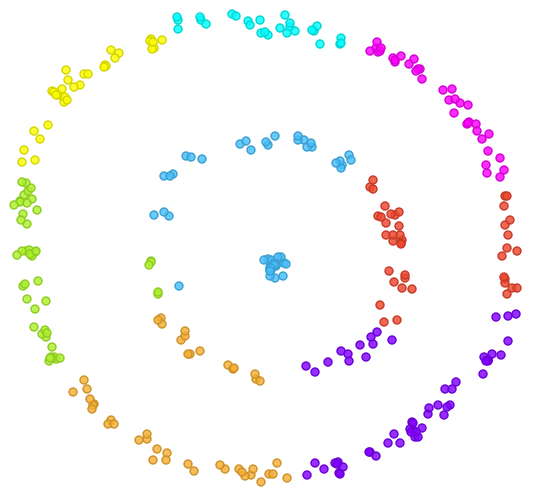
\includegraphics[width=\columnwidth]{results/circular_wsbm.png}
        \caption{WSBM}
        \label{fig:synthetic_ina}
    \end{subfigure}
    \caption{Different clusterings for the Circles dataset.}\label{fig:results_circular}
\end{figure}

To attempt to visually understand how the approaches differ, we visualize the synthetic datasets (we do this for the synthetic datasets as they are inherently two dimensional and thus easily visualized). We show the labellings for the Circles datasets (see Figure~\ref{fig:results_circular}) and the Two Moons dataset (see Figure~\ref{fig:results_moons}).

\begin{figure}[h]
    \centering
    \begin{subfigure}[c]{0.48\columnwidth}
        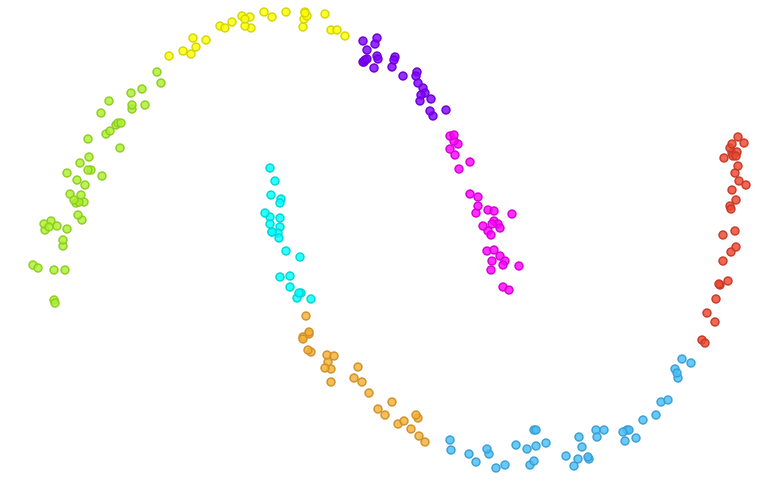
\includegraphics[width=\columnwidth]{results/moons_hc.png}
        \caption{k-means}
        \label{fig:synthetic_two_moons}
    \end{subfigure}
    ~
    \begin{subfigure}[c]{0.48\columnwidth}
        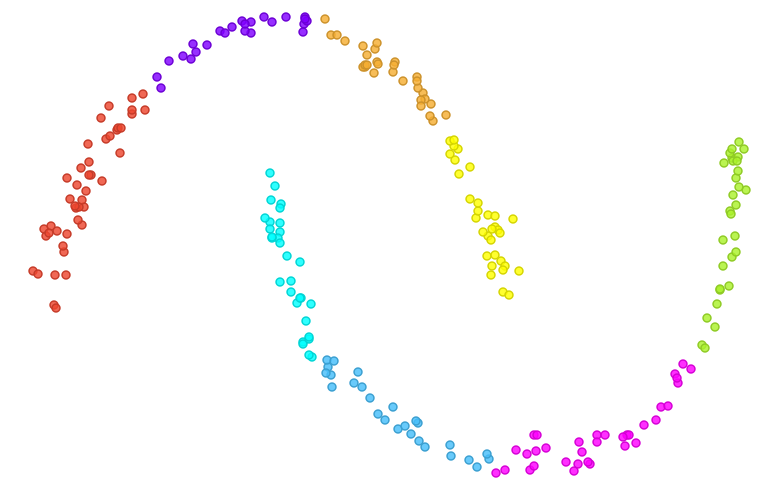
\includegraphics[width=\columnwidth]{results/moons_kmeans.png}
        \caption{Hierarchical clustering}
        \label{fig:synthetic_circles}
    \end{subfigure}
    ~
    \begin{subfigure}[c]{0.48\columnwidth}
        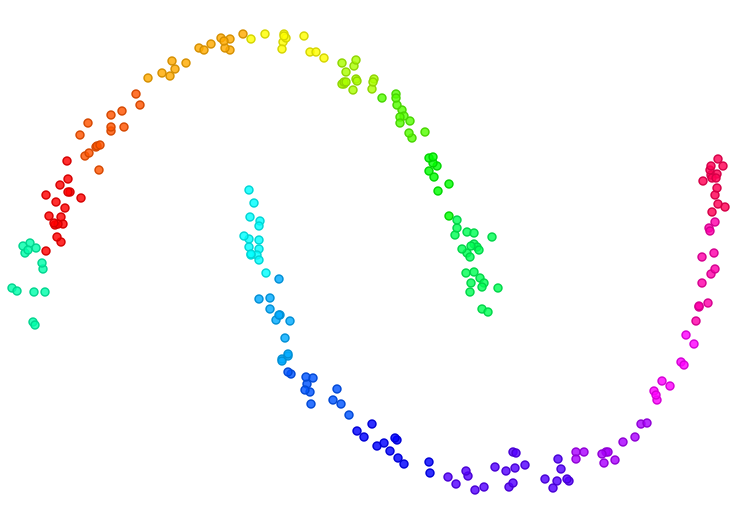
\includegraphics[width=\columnwidth]{results/moons_sbm.png}
        \caption{SBM with thresholding}
        \label{fig:synthetic_ina}
    \end{subfigure}
    ~
    \begin{subfigure}[c]{0.48\columnwidth}
        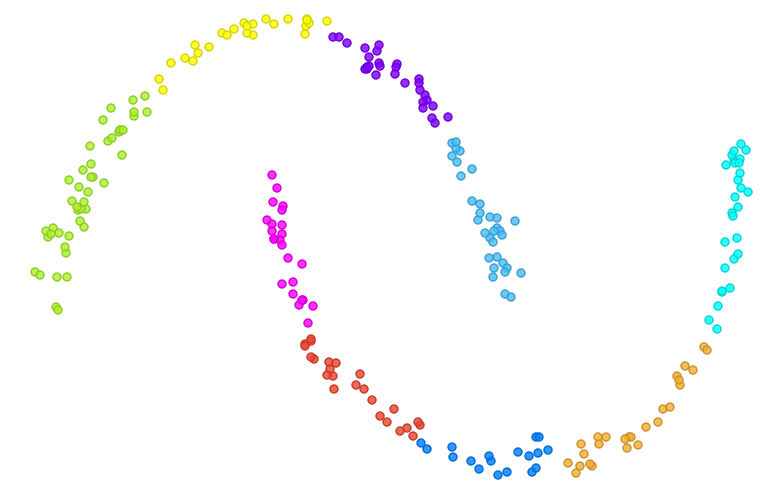
\includegraphics[width=\columnwidth]{results/moons_wsbm.png}
        \caption{WSBM}
        \label{fig:synthetic_ina}
    \end{subfigure}
    \caption{Different clusterings for the Two Moons dataset.}\label{fig:results_moons}
\end{figure}

It is clear from the images that there are no apparent differences between hierarchical clustering, k-means and the WSBM. We again notice that the SBM has produced a very large number of clusters, however the clusters seem very similar to those produced by the other methods.

The poor results could in part be explained by the fact that we are trying to optimize the silhouette score. However, the silhouette score may not be the best indicator of our synthetic datasets e.g. circles, since the silhouette takes into account the mean distance to all nodes in the same cluster. We can imagine that this does not bode well for this particular dataset since the points that should be part of the same cluster can be very far apart (on opposite sides of the outer circle). Trying to maximize a different score e.g. the NMI might produce better results, but as already mentioned, we can only do this when we already know the true labels of the data, therefore this is not useful for unsupervised learning tasks.

Different evaluation metrics would produce different results and one may not be appropriate in every scenario. The best selection of the evaluation metric can rarely be known in advance. This is due to the fact that clustering is an ill-defined problem since the results of clustering is usually up for interpretation.

\section{Conclusion}

In the presented work, we study stochastic block models and their generalization for data clustering. We show that a naive approach with thresholding does not perform as consistently as other methods. On the other hand, weighted stochastic block models achieve state-of-the-art results. However, we do not observe a significant improvement in the quality of the discovered clusters. In addition, the proposed method does not overcome the problem of automatically inferring the correct number of clusters. We observe that different similarity metrics used in the graph induction step do not have a large impact on the results. The analysis of this work can be extended by comparing our results with other community detection methods and using other approaches for optimizing the cluster quality.


\bibliographystyle{ieeetr}
\bibliography{references}


\begin{table*}[t]
  \centering
  \begin{tabular}{c | c | c c c | c}
    Dataset & Method & Silhouette & NMI & ARI & clusters \\ \hline
    Iris & k-means & \textbf{0.6808} & 0.6793 & 0.5399 & 2 \\
    Iris & Hierarchical clustering & \textbf{0.6864} & \textbf{0.7612} & \textbf{0.5681} & 2 \\
    Iris & SBM (Manhattan) & 0.3916 & 0.6752 & 0.5703 & 7 \\
    Iris & SBM (Euclidean) & 0.3855 & 0.6283 & 0.5517 & 7 \\
    Iris & SBM (Chebyshev) & 0.3889 & 0.6661 & \textbf{0.5673} & 6 \\
    Iris & WSBM (Manhattan) & \textbf{0.6864} & \textbf{0.7612} & \textbf{0.5681} & 2 \\
    Iris & WSBM (Euclidean) & \textbf{0.6864} & \textbf{0.7612} & \textbf{0.5681} & 2 \\
    Iris & WSBM (Chebyshev) & \textbf{0.6864} & \textbf{0.7612} & \textbf{0.5681} & 2 \\

    \hline
    Ecoli & k-means & 0.4303 & 0.6548 & 0.6860 & 4 \\
    Ecoli & Hierarchical clustering & 0.4166 & 0.6537 & 0.6575 & 4 \\
    Ecoli & SBM (Manhattan) & 0.0694 & 0.4821 & 0.1801 & 20 \\
    Ecoli & SBM (Euclidean) & 0.1458 & 0.1964 & -0.0182 & 3 \\
    Ecoli & SBM (Chebyshev) & \textbf{0.5524} & 0.2057 & 0.0380 & 2 \\
    Ecoli & WSBM (Manhattan) & 0.4263 & \textbf{0.6827} & \textbf{0.7261} & 4 \\
    Ecoli & WSBM (Euclidean) & 0.4288 & \textbf{0.6860} & \textbf{0.7310} & 4 \\
    Ecoli & WSBM (Chebyshev) & 0.4115 & 0.6425 & 0.6803 & 4 \\

    \hline
    Zoo & k-means & 0.4177 & 0.8172 & \textbf{0.8418} & 6 \\
    Zoo & Hierarchical clustering & \textbf{0.4288} & \textbf{0.8485} & \textbf{0.8483} & 7 \\
    Zoo & SBM (Manhattan) & 0.3811 & \textbf{0.8503} & 0.8137 & 5 \\
    Zoo & SBM (Euclidean) & 0.3999 & 0.8011 & 0.8089 & 5 \\
    Zoo & SBM (Chebyshev) & 0.3065 & 0.4778 & 0.3143 & 3 \\
    Zoo & WSBM (Manhattan) & 0.3191 & 0.7939 & 0.5243 & 11 \\
    Zoo & WSBM (Euclidean) & 0.3229 & 0.7481 & 0.5077 & 10 \\
    Zoo & WSBM (Chebyshev) & 0.3317 & 0.6016 & 0.4964 & 4 \\

    \hline
    Glass & k-means & \textbf{0.5891} & \textbf{0.4409} & \textbf{0.2549} & 4 \\
    Glass & Hierarchical clustering & \textbf{0.5888} & 0.3953 & 0.2311 & 4 \\
    Glass & SBM (Manhattan) & 0.1187 & 0.3546 & 0.1308 & 9 \\
    Glass & SBM (Euclidean) & 0.1042 & 0.3662 & 0.1619 & 8 \\
    Glass & SBM (Chebyshev) & 0.3398 & 0.3615 & 0.2345 & 5 \\
    Glass & WSBM (Manhattan) & 0.3864 & 0.2303 & 0.1368 & 2 \\
    Glass & WSBM (Euclidean) & 0.4401 & 0.2811 & 0.1898 & 2 \\
    Glass & WSBM (Chebyshev) & 0.5446 & 0.3612 & 0.2259 & 2 \\

    \hline
    Movements & k-means & \textbf{0.2399} & 0.4750 & 0.2385 & 8 \\
    Movements & Hierarchical clustering & \textbf{0.2400} & 0.5219 & 0.2241 & 9 \\
    Movements & SBM (Manhattan) & -0.0842 & 0.1402 & 0.0052 & 2 \\
    Movements & SBM (Euclidean) & 0.1497 & 0.6213 & \textbf{0.3114} & 24 \\
    Movements & SBM (Chebyshev) & 0.1094 & \textbf{0.6357} & 0.2575 & 37 \\
    Movements & WSBM (Manhattan) & -0.0148 & 0.0923 & 0.0074 & 2 \\
    Movements & WSBM (Euclidean) & 0.1975 & 0.2579 & 0.0639 & 2 \\
    Movements & WSBM (Chebyshev) & 0.0846 & 0.4798 & 0.2517 & 7 \\


    \hline
    Two Moons & k-means & \textbf{0.5753} & 0.5795 & 0.2533 & 8 \\
    Two Moons & Hierarchical clustering & \textbf{0.5717} & 0.5807 & 0.2581 & 8 \\
    Two Moons & SBM (Manhattan) & 0.5293 & 0.4944 & 0.1180 & 18 \\
    Two Moons & SBM (Euclidean) & 0.5489 & 0.5162 & 0.1486 & 14 \\
    Two Moons & SBM (Chebyshev) & 0.4732 & 0.4937 & 0.1198 & 19 \\
    Two Moons & WSBM (Manhattan) & 0.5692 & 0.5800 & 0.2550 & 8 \\
    Two Moons & WSBM (Euclidean) & 0.5656 & 0.5654 & 0.2316 & 9 \\
    Two Moons & WSBM (Chebyshev) & 0.5377 & \textbf{0.6227} & \textbf{0.3322} & 6 \\
    \hline
    INA & k-means & \textbf{0.5466} & \textbf{0.8238} & \textbf{0.7538} & 2 \\
    INA & Hierarchical clustering  & \textbf{0.5466} & \textbf{0.8238} & \textbf{0.7538} & 2 \\
    INA & SBM (Manhattan) & 0.4015 & 0.5468 & 0.1140 & 32 \\
    INA & SBM (Euclidean) & 0.3780 & 0.5458 & 0.1128 & 33 \\
    INA & SBM (Chebyshev) & 0.2946 & 0.5320 & 0.1132 & 35 \\
    INA & WSBM (Manhattan)  & \textbf{0.5466} & \textbf{0.8238} & \textbf{0.7538} & 2 \\
    INA & WSBM (Euclidean)  & \textbf{0.5466} & \textbf{0.8238} & \textbf{0.7538} & 2 \\
    INA & WSBM (Chebyshev)  & \textbf{0.5466} & \textbf{0.8238} & \textbf{0.7538} & 2 \\

    \hline
    Circular & k-means & 0.4279 & 0.2706 & 0.0747 & 7 \\
    Circular & Hierarchical clustering & 0.4045 & 0.3324 & 0.0813 & 9 \\
    Circular & SBM (Manhattan) & 0.5485 & 0.4901 & 0.0666 & 28 \\
    Circular & SBM (Euclidean) & 0.5257 & 0.4941 & 0.0704 & 27 \\
    Circular & SBM (Chebyshev) & \textbf{0.5635} & \textbf{0.4977} & 0.0751 & 26 \\
    Circular & WSBM (Manhattan) & 0.4178 & 0.3335 & 0.0894 & 8 \\
    Circular & WSBM (Euclidean) & 0.4264 & 0.3281 & 0.0846 & 8 \\
    Circular & WSBM (Chebyshev) & 0.4124 & 0.3261 & \textbf{0.1143} & 6 \\


  \end{tabular}
  \caption{Results}
  \label{tab:results_full}
\end{table*}




%\begin{table*}[t]
%  \centering
%  \begin{tabular}{c | c | c c c c}
%    Dataset & Method & Silhouette & NMI & ARI & clusters \\ \hline

%    iris & WSBM (Manhattan) & 0.5171 & 0.7206 & \textbf{0.6906} & 3 \\
%    iris & WSBM (Euclidean) & 0.4757 & 0.6068 & 0.5167 & 3 \\
%    iris & WSBM (Chebyshev) & 0.4932 & 0.6174 & 0.5237 & 3 \\

%    \hline

%    ecoli & WSBM (Manhattan) & 0.2022 & 0.5724 & 0.4363 & 8 \\
%    ecoli & WSBM (Euclidean) & 0.1584 & 0.5600 & 0.4267 & 8 \\
%    ecoli & WSBM (Chebyshev) & 0.1744 & 0.5540 & 0.4233 & 8 \\
%    \hline

%    zoo & WSBM (Manhattan) & 0.1258 & 0.6229 & 0.3602 & 7 \\
%    zoo & WSBM (Euclidean) & 0.2060 & 0.6716 & 0.4700 & 7 \\
%    zoo & WSBM (Chebyshev) & 0.2100 & \textbf{0.6189} & 0.4046 & 7 \\

%    \hline
%    Two Moons & WSBM (Manhattan) & 0.4686 & 0.2063 & \textbf{0.2675} & 2 \\
%    Two Moons & WSBM (Euclidean) & 0.4686 & 0.2063 & \textbf{0.2675} & 2 \\
%    Two Moons & WSBM (Chebyshev) & 0.4686 & 0.2063 & 0.2675 & 2 \\

%    \hline

%    INA & WSBM (Manhattan) & 0.4463 & 0.7529 & 0.6966 & 3 \\
%    INA & WSBM (Euclidean) & 0.4463 & 0.7543 & 0.6993 & 3 \\
%    INA & WSBM (Chebyshev) & 0.4464 & 0.7536 & 0.6979 & 3 \\

%    \hline
%    circular & WSBM (Manhattan) & 0.2619 & 0.2367 & \textbf{0.1167} & 3 \\
%    circular & WSBM (Euclidean) & 0.2527 & 0.2906 & \textbf{0.1846} & 3 \\
%    circular & WSBM (Chebyshev) & 0.2758 & 0.3082 & \textbf{0.2036} & 3 \\

%  \end{tabular}
%  \caption{Results for known number of clusters}
%  \label{tab:results_known}
%\end{table*}

%% This figure may be completely pointless since it will be clear from the results table that distances have little effect on SBM threshold performance
%% TODO rerun this code and make the legend nicer (should be in format: Inverse Chebyshev)
%\begin{figure}[ht]
    %\centering
    %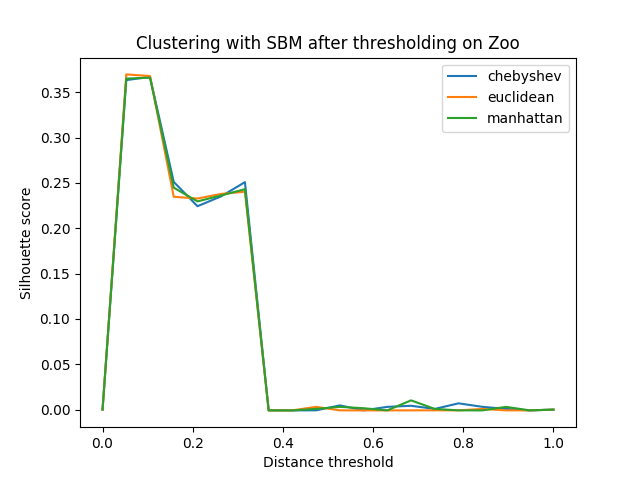
\includegraphics[width=\columnwidth]{results/threshold_clustering_metrics_zoo.png}
    %\caption{Comparison of SBM performance using the threshold method for different distance metrics.}
%    \label{fig:threshold_sbm_iris_metrics}
%\end{figure}


% needed in second column of first page if using \IEEEpubid
%\IEEEpubidadjcol

% An example of a floating figure using the graphicx package.
% Note that \label must occur AFTER (or within) \caption.
% For figures, \caption should occur after the \includegraphics.
% Note that IEEEtran v1.7 and later has special internal code that
% is designed to preserve the operation of \label within \caption
% even when the captionsoff option is in effect. However, because
% of issues like this, it may be the safest practice to put all your
% \label just after \caption rather than within \caption{}.
%
% Reminder: the "draftcls" or "draftclsnofoot", not "draft", class
% option should be used if it is desired that the figures are to be
% displayed while in draft mode.
%
%\begin{figure}[!t]
%\centering
%\includegraphics[width=2.5in]{myfigure}
% where an .eps filename suffix will be assumed under latex,
% and a .pdf suffix will be assumed for pdflatex; or what has been declared
% via \DeclareGraphicsExtensions.
%\caption{Simulation Results}
%\label{fig_sim}
%\end{figure}

% Note that IEEE typically puts floats only at the top, even when this
% results in a large percentage of a column being occupied by floats.


% An example of a double column floating figure using two subfigures.
% (The subfig.sty package must be loaded for this to work.)
% The subfigure \label commands are set within each subfloat command, the
% \label for the overall figure must come after \caption.
% \hfil must be used as a separator to get equal spacing.
% The subfigure.sty package works much the same way, except \subfigure is
% used instead of \subfloat.
%
%\begin{figure*}[!t]
%\centerline{\subfloat[Case I]\includegraphics[width=2.5in]{subfigcase1}%
%\label{fig_first_case}}
%\hfil
%\subfloat[Case II]{\includegraphics[width=2.5in]{subfigcase2}%
%\label{fig_second_case}}}
%\caption{Simulation results}
%\label{fig_sim}
%\end{figure*}
%
% Note that often IEEE papers with subfigures do not employ subfigure
% captions (using the optional argument to \subfloat), but instead will
% reference/describe all of them (a), (b), etc., within the main caption.


% An example of a floating table. Note that, for IEEE style tables, the
% \caption command should come BEFORE the table. Table text will default to
% \footnotesize as IEEE normally uses this smaller font for tables.
% The \label must come after \caption as always.
%
%\begin{table}[!t]
%% increase table row spacing, adjust to taste
%\renewcommand{\arraystretch}{1.3}
% if using array.sty, it might be a good idea to tweak the value of
% \extrarowheight as needed to properly center the text within the cells
%\caption{An Example of a Table}
%\label{table_example}
%\centering
%% Some packages, such as MDW tools, offer better commands for making tables
%% than the plain LaTeX2e tabular which is used here.
%\begin{tabular}{|c||c|}
%\hline
%One & Two\\
%\hline
%Three & Four\\
%\hline
%\end{tabular}
%\end{table}


% Note that IEEE does not put floats in the very first column - or typically
% anywhere on the first page for that matter. Also, in-text middle ("here")
% positioning is not used. Most IEEE journals use top floats exclusively.
% Note that, LaTeX2e, unlike IEEE journals, places footnotes above bottom
% floats. This can be corrected via the \fnbelowfloat command of the
% stfloats package.








% if have a single appendix:
%\appendix[Proof of the Zonklar Equations]
% or
%\appendix  % for no appendix heading
% do not use \section anymore after \appendix, only \section*
% is possibly needed

% use appendices with more than one appendix
% then use \section to start each appendix
% you must declare a \section before using any
% \subsection or using \label (\appendices by itself
% starts a section numbered zero.)
%


%\appendices
%\section{Proof of the First Zonklar Equation}
%\blindtext

% use section* for acknowledgement
%\section*{Acknowledgment}


%The authors would like to thank...


% Can use something like this to put references on a page
% by themselves when using endfloat and the captionsoff option.
%\ifCLASSOPTIONcaptionsoff
%  \newpage
%\fi



% trigger a \newpage just before the given reference
% number - used to balance the columns on the last page
% adjust value as needed - may need to be readjusted if
% the document is modified later
%\IEEEtriggeratref{8}
% The "triggered" command can be changed if desired:
%\IEEEtriggercmd{\enlargethispage{-5in}}

% references section

% can use a bibliography generated by BibTeX as a .bbl file
% BibTeX documentation can be easily obtained at:
% http://www.ctan.org/tex-archive/biblio/bibtex/contrib/doc/
% The IEEEtran BibTeX style support page is at:
% http://www.michaelshell.org/tex/ieeetran/bibtex/
%\bibliographystyle{IEEEtran}
% argument is your BibTeX string definitions and bibliography database(s)
%\bibliography{IEEEabrv,../bib/paper}
%
% <OR> manually copy in the resultant .bbl file
% set second argument of \begin to the number of references
% (used to reserve space for the reference number labels box)
%\begin{thebibliography}{1}

%\bibitem{IEEEhowto:kopka}
%H.~Kopka and P.~W. Daly, \emph{A Guide to \LaTeX}, 3rd~ed.\hskip 1em plus
%  0.5em minus 0.4em\relax Harlow, England: Addison-Wesley, 1999.

%\end{thebibliography}

% biography section
%
% If you have an EPS/PDF photo (graphicx package needed) extra braces are
% needed around the contents of the optional argument to biography to prevent
% the LaTeX parser from getting confused when it sees the complicated
% \includegraphics command within an optional argument. (You could create
% your own custom macro containing the \includegraphics command to make things
% simpler here.)
%\begin{biography}[{\includegraphics[width=1in,height=1.25in,clip,keepaspectratio]{mshell}}]{Michael Shell}
% or if you just want to reserve a space for a photo:

\begin{IEEEbiography}[{\includegraphics[width=1in,height=1.25in,clip,keepaspectratio]{picture}}]{John Doe}
\blindtext
\end{IEEEbiography}

% You can push biographies down or up by placing
% a \vfill before or after them. The appropriate
% use of \vfill depends on what kind of text is
% on the last page and whether or not the columns
% are being equalized.

%\vfill

% Can be used to pull up biographies so that the bottom of the last one
% is flush with the other column.
%\enlargethispage{-5in}

%\appendix
%\section{Synthetic datasets}
%\begin{figure}[H]
%    \centering
%    \begin{subfigure}[c]{0.3\columnwidth}
%        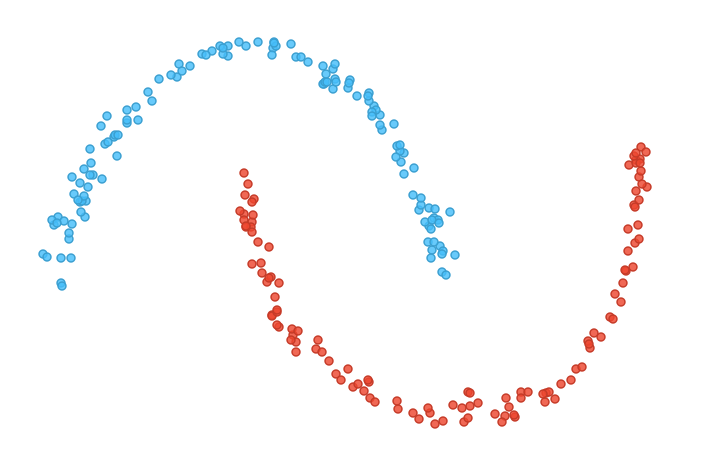
\includegraphics[width=\columnwidth]{images/moons.png}
%        \caption{The two moons dataset}
%        \label{fig:synthetic_two_moons}
%    \end{subfigure}
%    ~
%    \begin{subfigure}[c]{0.3\columnwidth}
%        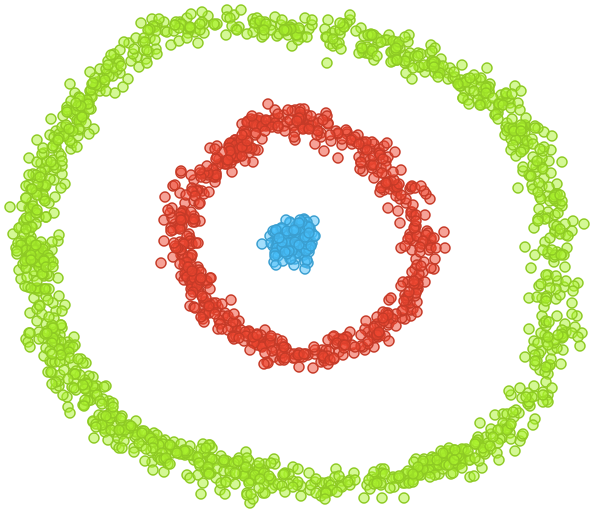
\includegraphics[width=\columnwidth]{images/circles.png}
%        \caption{The circles dataset}
%        \label{fig:synthetic_circles}
%    \end{subfigure}
%    ~
%    \begin{subfigure}[c]{0.3\columnwidth}
%        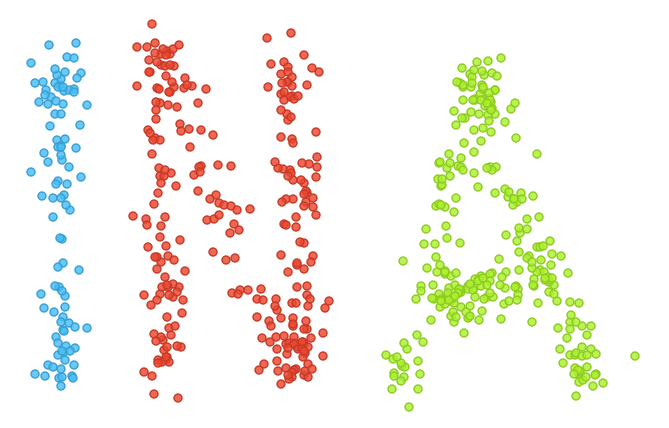
\includegraphics[width=\columnwidth]{images/ina.png}
%        \caption{The INA dataset}
%        \label{fig:synthetic_ina}
%    \end{subfigure}
%    \caption{Synthetic datasets}\label{fig:synthetic_datasets}
%\end{figure}


% that's all folks
\end{document}


